%!TEX root = ../document.tex
\chapter{Verwendete Tools}
Es folgt eine kurze Übersicht der Tools, die in den Beispielen mehrfach eingesetzt werden. Hier wird jeweils der Zweck des Tools und die Bedienung kurz demonstriert.

\section{Wireshark}

% TODO entweder rausnehmen oder ergänzen.
Wireshark kann von \url{https://www.wireshark.org/#download} heruntergeladen werden.

\section{Kommandozeilenprogramme}
\subsection{ifconfig}

\colorbox{altgray}{\lstinline|ifconfig|} ist ein Kommandozeilenprogramm unter Unix, das zur Konfiguration und Steuerung von IP-Netzwerkschnittstellen dient. Der Name steht für \enquote{interface configurator}.

Abbildung \ref{img:ifconfig} zeigt beispielhaft eine Ausgabe des Programms. Die relevantesten Informationen wie IP-Adresse, MAC und Interfacenamen wurden in der Grafik hervorgehoben.

\begin{figure}[H]
	\centering
	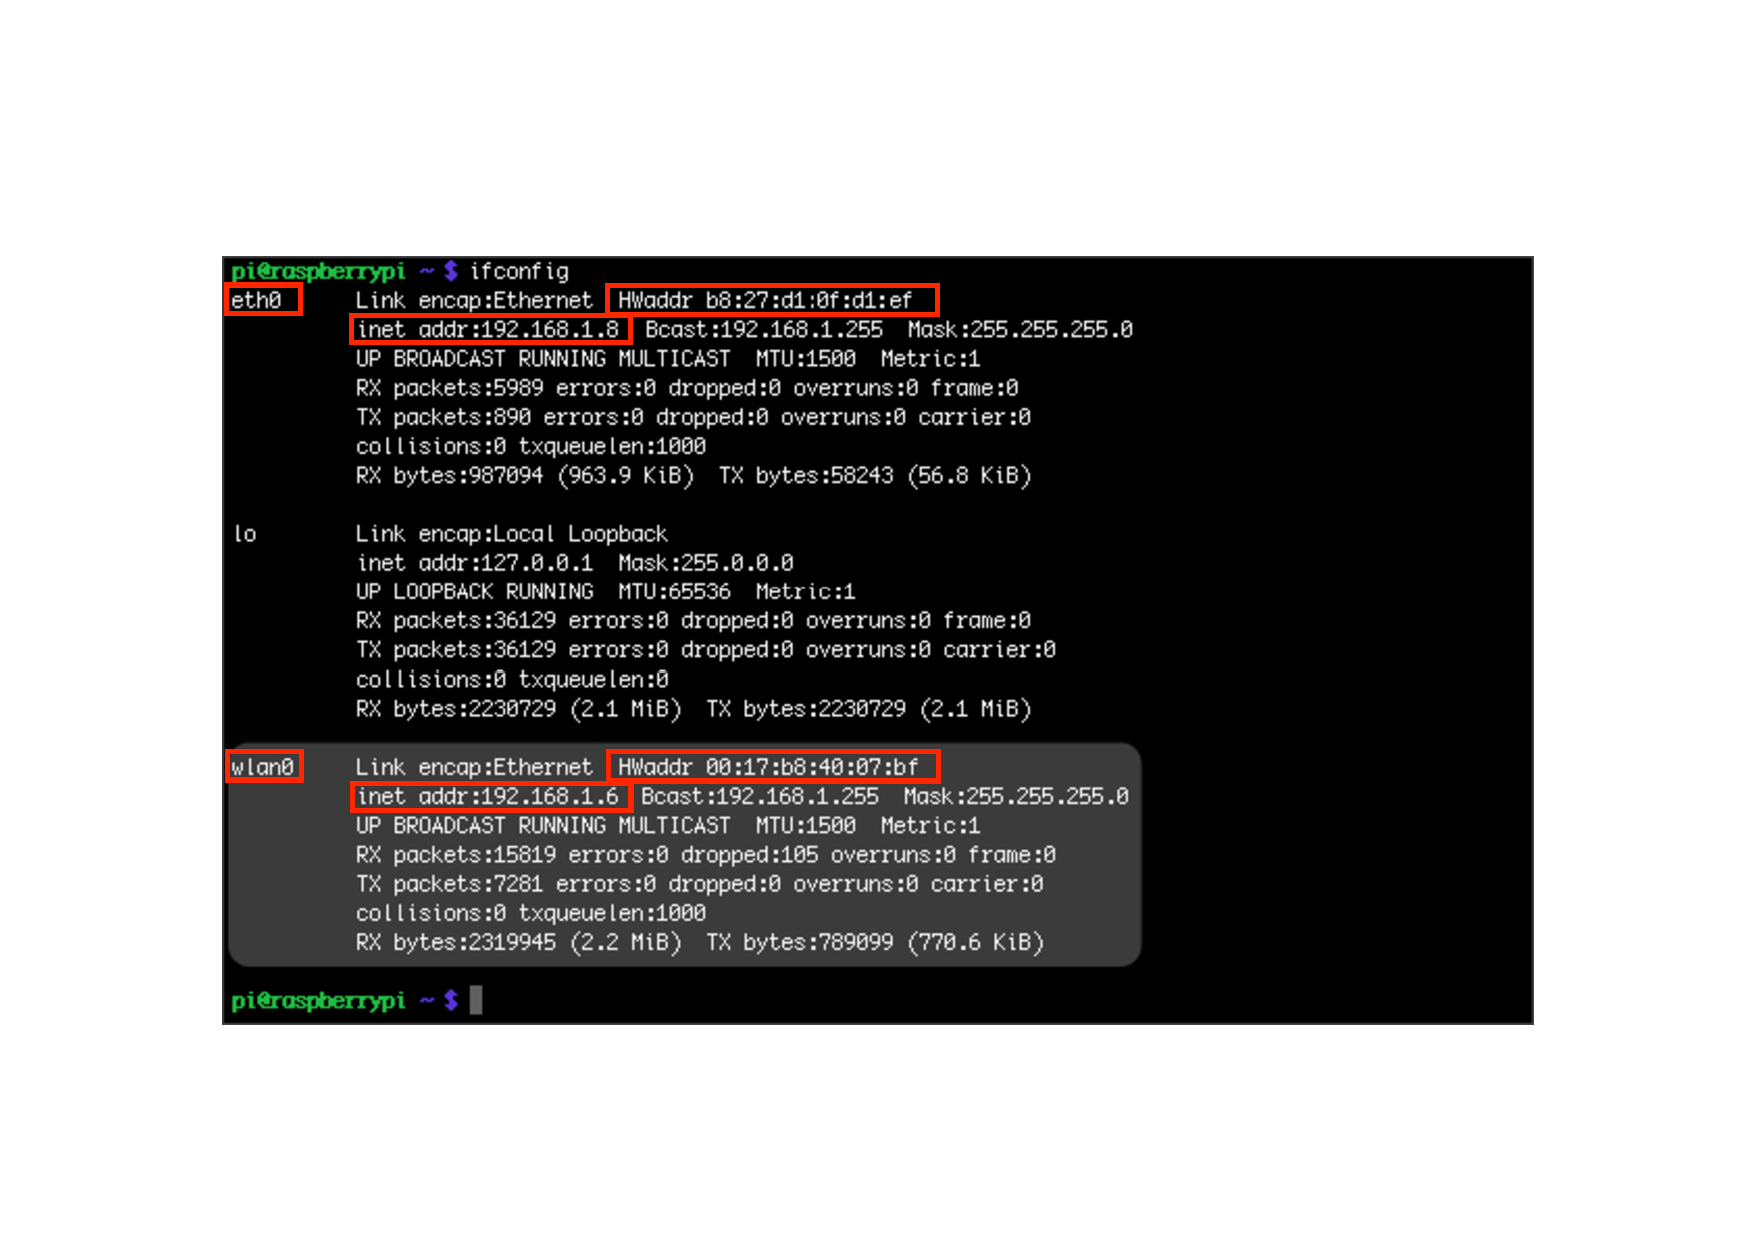
\includegraphics[width=1\textwidth]{images/ifconfig.pdf}
	\caption{Beispielausgabe ifconfig}
	\label{img:ifconfig}
\end{figure}

\subsection{aircrack-ng}
\colorbox{altgray}{\lstinline|aircrack-ng|} ist eine komplette Suite von Tools zur Beurteilung der WLAN-Sicherheit. Es wird hier unter anderem zum Cracken der WEP-Verschlüsselung verwendet. Ebenso liefert die Suite Tools zum Monitoring, Angreifen und Testen von WLAN-Netzwerken. Weitere Informationen findet man in der Dokumentation der \colorbox{altgray}{\lstinline|aircrack-ng|}-Suite auf \colorbox{altgray}{\lstinline|http://www.aircrack-ng.org/doku.php|}. Dort kann man auch die verschiedenen Tools und ihre Funktionen einsehen.

\subsection{mdk3}
MDK oder auch Murder Death Kill ist ein Tool, um bei IEEE 802.11-Protokollschwächen aufzudecken. Es wird in dieser Arbeit für DoS Angriffe verwendet. Weitere Informationen über die Funktionsweise findet man unter \colorbox{altgray}{\lstinline|mdk3 --help|}.

\subsection{crunch}
Mit \colorbox{altgray}{\lstinline|crunch|} lassen sich Bruteforce-Attacken mit Wordlists durchführen, um zum Beispiel WPA/WPA2 Passwörter zu knacken. Weitere Informationen zur Bedienung findet man unter \colorbox{altgray}{\lstinline|https://www.wardriving-forum.de/wiki/Crunch_Wordlist_Tutorial|}.


\subsection{reaver und wash}
\colorbox{altgray}{\lstinline|reaver|} ist ein Brute-Force-Tool, welches zum Knacken von WPS-PIN-Verfahren genutzt und somit der WPA/WPA2-PSK extrahiert werden kann. Zu \colorbox{altgray}{\lstinline|reaver|} gehört auch das Kommandozeilenprogramm \colorbox{altgray}{\lstinline|wash|}. Dieses hat im Prinzip nur den einen Zweck, herauszufinden welche WLANs die Authentifizierung per WPS zulassen, und ob WPS gerade aktiv ist. Weitere Informationen zu reaver lassen sich einfach durch die Eingabe von \colorbox{altgray}{\lstinline|reaver --help|} in der Kommandozeile aufrufen.

\subsection{bully}

\colorbox{altgray}{\lstinline|bully|} ist ein weiteres Brute-Force-Tool für WPS, dass hier als Alternative für \colorbox{altgray}{\lstinline|reaver|} angewendet wird. Über \colorbox{altgray}{\lstinline|bully --help|} kann man in der Kommandozeile weitere Informationen zu den Parametern einsehen.

\subsection{hashcat}
\colorbox{altgray}{\lstinline|Hashcat|} ist als Open Source Software konzipiert und der schnellste Passwortcracker der zur Zeit erhältlich ist. Außerdem nutzt diese Software die GPU einer dedizierte Grafikkarte für den Cracking-Vorgang. Weitere Informationen lassen sich entweder in der Kommandozeile über \colorbox{altgray}{\lstinline|hashcat --help|} oder auf der \colorbox{altgray}{\lstinline|hashcat|}-Seite unter \colorbox{altgray}{\lstinline|https://hashcat.net/wiki/doku.php?id=hashcat|} einsehen.

\subsection{OpenSSL}
OpenSSL ist ein Toolkit und eine Bibliothek rund um die Erzeugung und Verwaltung von Zertifikaten und Schlüsseldateien. Zudem stellt sie eine Implementierung verschiedener Netzwerkprotokolle rund um SSL und TLS bereit. OpenSSL wird in Webservern wie Apache und nginx eingesetzt.

\subsection{Nmap}
Nmap ist ein Portscanner -- er ermöglicht es, in einem Netzwerk offene UDP und TCP Ports aufzuspüren und bietet auch eine Erkennung der laufenden Dienste sowie des verwendeten Betriebssystems an. Als Alternative zum kommandozeilenbasierten Nmap existiert mit Zenmap auch ein darauf aufbauendes Tool mit graphischer Oberfläche und gleichem Funktionsumfang.

\subsection{hping3}
hping ist ein kommandozeilen TCP/IP-Paketerzeuger und Analyst. hping unterstützt TCP, UDP, ICMP und RAW-IP Protokolle. hping wird unter anderem für Firewalltests und Netzwerktests verwendet.

\subsection{Metasploit}

Das Metasploit-Framework ist eine Sammlung von konfigurierbaren Exploits, welches mit dem Kommando \bashCommand{msfconsole} gestartet werden kann. Zur Dokumentation der Ergebnisse -- etwa im Rahmen eines Penetrationtestings -- kann eine PostgreSQL-Datenbank angebunden werden.

\subsection{arp}
\colorbox{altgray}{\lstinline|arp|} ist ein Kommandozeilenprogramm zum Auslesen und Verändern des ARP-Caches. Es wird hier verwendet, um die ARP-Tabelle vor und nach einem Angriff darzustellen. Mit Hilfe von \colorbox{altgray}{\lstinline|man arp|} können zusätzliche Informationen und die zur Verfügung stehenden Parameter nachgelesen werden.

\subsection{sslstrip}
Dieses Tool wird zur Demonstration der SSLStrip Attacke verwendet. Dabei werden HTTPS-Verbindungen des Opfers auf HTTP-Verbindungen umgeleitet wodurch der Datenverkehr mitgelesen werden kann. Das Tool wurde von Moxie Marlinspake entwickelt und unter \colorbox{altgray}{\lstinline|https://moxie.org/software/sslstrip/ |} können weitere Informationen eingesehen werden.

\subsection{iptables}
Mit Hilfe von \colorbox{altgray}{\lstinline|iptables|} können Regeln zur Konfiguration der Firewall erstellt und bearbeitet werden. Unter \colorbox{altgray}{\lstinline|man iptables|} ist eine sehr ausführliche Dokumentation zur Benutzung zu finden.

\subsection{sysctl}
\colorbox{altgray}{\lstinline|sysctl|} ist ein Werkzeug zur Veränderung von Kernelparameter während der Laufzeit. Dabei können alle Parameter bearbeitet werden, die unter proc/sys/ aufgelistet sind. Zusätzliche Informationen werden bei der Ausführung von \colorbox{altgray}{\lstinline|man sysctl|} ausgegeben.

\subsection{GNU Compiler Collection}
Die GNU Compiler Collection bietet Compiler für verschiedene Programmiersprachen und unterschiedliche Betriebssystemen. Hier wird der C-Compiler zusammen mit dem GNU Debugger verwendet. Auf der Homepage \colorbox{altgray}{\lstinline|https://gcc.gnu.org|} kann man sich über die unterstützten Sprachen und Betriebssysteme als auch über die neuesten Releases informieren.

\subsection{hostapd}
\colorbox{altgray}{\lstinline|hostapd|} ist ein WLAN-Deamon/Dienst, der auch auf linuxbetriebenen Routern zu finden ist. \colorbox{altgray}{\lstinline|hostapd|} implementiert nach IEEE 802.11 das Access-Point-Management, IEEE 802.1X/WPA/WPA2/EAP Authentikatoren, eine RADIUS Client, EAP Server und RADIUS Authentifizierungsserver.
\subsection{wifiphisher}
\colorbox{altgray}{\lstinline|wifiphisher|} ist ein Python-Kommandozeilenprogramm welches konfigurierbare Wifi-Phishing-Angriffe zur Verfügung stellt. \colorbox{altgray}{\lstinline|wifiphisher|} baut Fake-Access-Points auf und liefert dazugehörige Phishing-Seiten um beispielsweise WLAN-Zugangskennwörter abzufragen.
